%%%%%%%%%%%%%%%%%%%%%%%%%%%%%%%%%%%%%%%%%
% baposter Landscape Poster
% LaTeX Template
% Version 1.0 (11/06/13)
%
% baposter Class Created by:
% Brian Amberg (baposter@brian-amberg.de)
%
% This template has been downloaded from:
% http://www.LaTeXTemplates.com
%
% License:
% CC BY-NC-SA 3.0 (http://creativecommons.org/licenses/by-nc-sa/3.0/)
%
%%%%%%%%%%%%%%%%%%%%%%%%%%%%%%%%%%%%%%%%%

%----------------------------------------------------------------------------------------
%	PACKAGES AND OTHER DOCUMENT CONFIGURATIONS
%----------------------------------------------------------------------------------------

\documentclass[landscape,a0paper,fontscale=0.285]{baposter} % Adjust the font scale/size here

\usepackage{graphicx} % Required for including images
\graphicspath{{figures/}} % Directory in which figures are stored

\usepackage{amsmath} % For typesetting math
\usepackage{amssymb} % Adds new symbols to be used in math mode

\usepackage{booktabs} % Top and bottom rules for tables
\usepackage{enumitem} % Used to reduce itemize/enumerate spacing
\usepackage{palatino} % Use the Palatino font
\usepackage[font=small,labelfont=bf]{caption} % Required for specifying captions to tables and figures

\usepackage{multicol} % Required for multiple columns
\setlength{\columnsep}{1.5em} % Slightly increase the space between columns
\setlength{\columnseprule}{0mm} % No horizontal rule between columns

\usepackage{tikz} % Required for flow chart
\usetikzlibrary{shapes,arrows} % Tikz libraries required for the flow chart in the template

\newcommand{\compresslist}{ % Define a command to reduce spacing within itemize/enumerate environments, this is used right after \begin{itemize} or \begin{enumerate}
\setlength{\itemsep}{1pt}
\setlength{\parskip}{0pt}
\setlength{\parsep}{0pt}
}

\definecolor{lightblue}{rgb}{0.145,0.6666,1} % Defines the color used for content box headers

\begin{document}

\begin{poster}
{
headerborder=closed, % Adds a border around the header of content boxes
colspacing=1em, % Column spacing
bgColorOne=white, % Background color for the gradient on the left side of the poster
bgColorTwo=white, % Background color for the gradient on the right side of the poster
borderColor=lightblue, % Border color
headerColorOne=black, % Background color for the header in the content boxes (left side)
headerColorTwo=lightblue, % Background color for the header in the content boxes (right side)
headerFontColor=white, % Text color for the header text in the content boxes
boxColorOne=white, % Background color of the content boxes
textborder=roundedleft, % Format of the border around content boxes, can be: none, bars, coils, triangles, rectangle, rounded, roundedsmall, roundedright or faded
eyecatcher=true, % Set to false for ignoring the left logo in the title and move the title left
headerheight=0.1\textheight, % Height of the header
headershape=roundedright, % Specify the rounded corner in the content box headers, can be: rectangle, small-rounded, roundedright, roundedleft or rounded
headerfont=\Large\bf\textsc, % Large, bold and sans serif font in the headers of content boxes
%textfont={\setlength{\parindent}{1.5em}}, % Uncomment for paragraph indentation
linewidth=2pt % Width of the border lines around content boxes
}
%----------------------------------------------------------------------------------------
%	TITLE SECTION 
%----------------------------------------------------------------------------------------
%
{
\includegraphics[height=4em]{nyu_long_logo.jpg}} % First university/lab logo on the left
{\bf\textsc{DOTA2 Match Result Prediction Based On Hero Lineups}\vspace{0.5em}} % Poster title
{\textsc{Team 509:\hspace{6pt} Zhaoyin Zhu and Shuang Zhou  }} % Author names and institution
{
\includegraphics[height=6em]{dota2_logo.jpg}} % First university/lab logo on the left

%----------------------------------------------------------------------------------------
%	Introduction
%----------------------------------------------------------------------------------------

\headerbox{Introduction}{name=objectives,column=0,row=0}{

Dota 2 is a free-to-play multiplayer online battle arena (MOBA) video game developed and published by Valve Corporation. Dota 2 is played in matches between two five-player teams, represented by the name "dire" and "radiant", each of which occupies a stronghold in a corner of the playing field. \\
A team wins by destroying the other side's "Ancient" building, located within the opposing stronghold. Each player controls one of 113 playable "Hero" characters that feature unique powers and styles of play. During a match, the player collects gold, items, and experience points for their Hero, while combating Heroes of the opposite team.
\vspace{0.3em} % When there are two boxes, some whitespace may need to be added if the one on the right has more content
}

%----------------------------------------------------------------------------------------
%	Motivation
%----------------------------------------------------------------------------------------

\headerbox{Objectives}{name=introduction,column=1,row=0,bottomaligned=objectives}{
With the purpose of proposing a programmatic strategy to pick out a lineup that puts a team in the driver seat before the match even begins, two capstones have been established:
\begin{itemize}
\item Predict the outcome of a match given only the lineups under the assumption that both sides perform around the same level.
\item In order to obtain a high winning rate, recommend a sequence of picks in response to another sequence of picks to simulate the actual hero selection stage. 
\end{itemize}
}

%----------------------------------------------------------------------------------------
%	RESULTS 1
%----------------------------------------------------------------------------------------

\headerbox{Methods}{name=results,column=2,span=2,row=0}{

\begin{multicols}{2}
	The outcome of this data is binary and defined as:
	\begin{displaymath}
	Y = \left\{
	\begin{array}{lr}
	1, \text{if radiant wins}\\
	0, \text{otherwise}
	\end{array}
	\right.
	\end{displaymath}
	In order to achieve desirable prediction accuracy, 3 types of features are included as potential predictors:\\ 
	Single heroes:
	\begin{align*}
	D_i &= \left\{
	\begin{array}{lr}
	1, \text{if dire has hero with id i}\\
	0, \text{otherwise}
	\end{array}
	\right.\\
		R_i &= \left\{
		\begin{array}{lr}
			1, \text{if radiant has hero with id i}\\
			0, \text{otherwise}
		\end{array}
		\right.
		\end{align*} 
	Joint combinations of two heroes on the same side	
	\begin{align*}
	D_iD_j &= \left\{
	\begin{array}{lr}
	1, \text{if dire has both hero i and hero j}\\
	0, \text{otherwise}
	\end{array}
	\right.\\
		R_iR_j &= \left\{
		\begin{array}{lr}
		1, \text{if radiant has both hero i and hero j}\\
		0, \text{otherwise}
		\end{array}
		\right.
		\end{align*} 
	Joint combinations of two heroes on the opposite side:	
	\begin{displaymath}
	D_iR_j = \left\{
	\begin{array}{lr}
	1, \text{if dire has hero i, radiant has hero j}\\
	0, \text{otherwise}
	\end{array}
	\right.
	\end{displaymath} 		
	The number of features in this case is slight larger than the number of instances, thus for parametric models such as Logistic Regression to work, model-free feature selection is required. This can be done based on the appearance frequency of each feature and Pearson product-moment correlation coefficients between each feature and the binary outcome. \\
	In modeling the data, both nonparametric methods (KNN, random forest) and parametric methods (SVM, logistic regression) can be used. In parametric models, penalized methods like LASSO and SCAD can be used as well. In order to evaluate the performance of different methods, the dataset will be randomly split into training set ($n_{training} = 10000$) and testing set ($n_{test = 2000}$). \\
\end{multicols}

}

%----------------------------------------------------------------------------------------
%	REFERENCES
%----------------------------------------------------------------------------------------

\headerbox{References}{name=references,column=0,above=bottom}{

[1] James, G., Witten, D., Hastie, T., \& Tibshirani, R. (2013). \emph{An introduction to statistical learning} (Vol. 112). New York: springer.
}
\headerbox{References}{name=references,column=1,above=bottom}{
	
	[2] Friedman, J., Hastie, T., \& Tibshirani, R. (2001). \emph{The elements of statistical learning} (Vol. 1). Springer, Berlin: Springer series in statistics.
}
%----------------------------------------------------------------------------------------
%	FUTURE RESEARCH
%----------------------------------------------------------------------------------------

\headerbox{Future Research}{name=futureresearch,column=2,span=2,aligned=references,above=bottom}{ % This block is as tall as the references block

\begin{multicols}{2}
A new patch will be released every few months that dramatically changes the balance of the game and thousands of games have been played everyday. We believe that a sliding window of new match history data could help maintain data relevancy. 

\end{multicols}
}



%----------------------------------------------------------------------------------------
%	CONCLUSION
%----------------------------------------------------------------------------------------

\headerbox{Recommendation Eigine}{name=conclusion,column=2,span=2,row=0,below=results,above=references}{	
	\begin{tabular}{ccc}

\includegraphics[width=6em,height=17em]{ok}
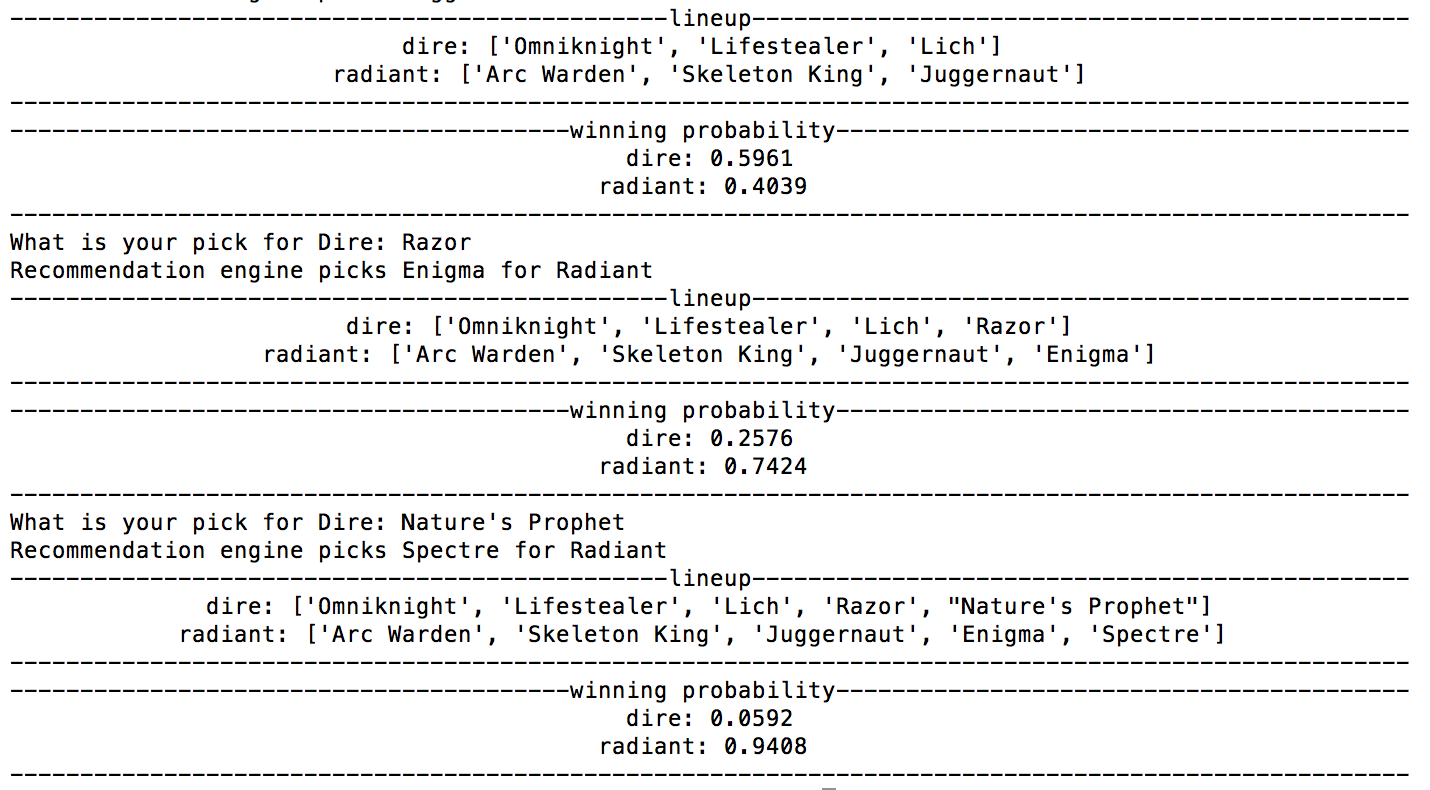
\includegraphics[height=17em]{result2}
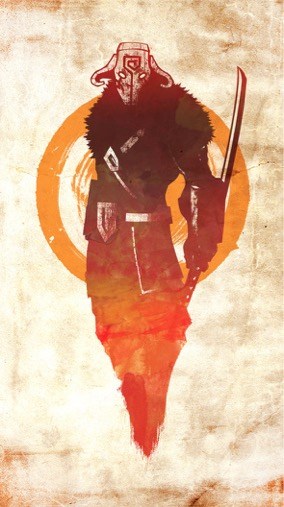
\includegraphics[width=6em,height=17em]{jugg}
	\end{tabular}

}

%----------------------------------------------------------------------------------------
%	MATERIALS AND METHODS
%----------------------------------------------------------------------------------------

\headerbox{Motivation}{name=method,column=0,below=objectives,bottomaligned=conclusion}{ % This block's bottom aligns with the bottom of the conclusion block

ESports are getting growing attention and popularity. In 2015, the fifth TI tounament (TI5) in Seattle had the largest prize pool in eSports history, with a total of \$10.9 million. Therefore, it is very worthwhile to research the strategies and tactics within the game to have a better chance against competitions,yet this is a very new ground awaiting discovery.\\
Each match in Dota starts with the players picking their heroes. This stage of a match is much more important than it seems, and very often a bad lineup will pretty much rule the team out. A lot of strategies can be applied during the banning and picking. To name a few, a team may want to ban the heroes that worked really
well for the opposing team before, or they want to counter a specific hero in the opposing
lineup by picking one that can contain it with a later pick, or they want to achieve a 1+1 > 2
effect by designing their lineup in a way that heroes supplement each other.  
}
%----------------------------------------------------------------------------------------
%	RESULTS 2
%----------------------------------------------------------------------------------------

\headerbox{Results}{name=results2,column=1,below=objectives,bottomaligned=conclusion}{ % This block's bottom aligns with the bottom of the conclusion block
After some trials, the number of appearances in the dataset has random effect on performance, that is, no obvious relation between the threshold we set and the accuracy we obtain is observed. The best cut-off point for Pearson correlation coefficients is 0.011. Furthermore, model-based penalized methods do not increase accuracy significantly.\\
The best performers among various models after feature selection is displayed in the following table,
\begin{center}
	\begin{tabular}{| c | c | c |}\hline
		Model & Training & Validation\\\hline
		Random Forest & 0.9967 & 0.6285 \\\hline
		SVM & 0.8403 & 0.6720 \\\hline
		Logistic Regression & 0.7861 & 0.6800 \\\hline
	\end{tabular}
\end{center}
Other trials are Decision Trees, KNN classifier and adaBoost. However, these models prove to be ill-suited for this dataset so we have omitted them in the table.

}

%----------------------------------------------------------------------------------------

\end{poster}

\end{document}